\begin{frame}
    \frametitle{Modelo de cámara Pinhole}
    
    \begin{figure}[!h]
        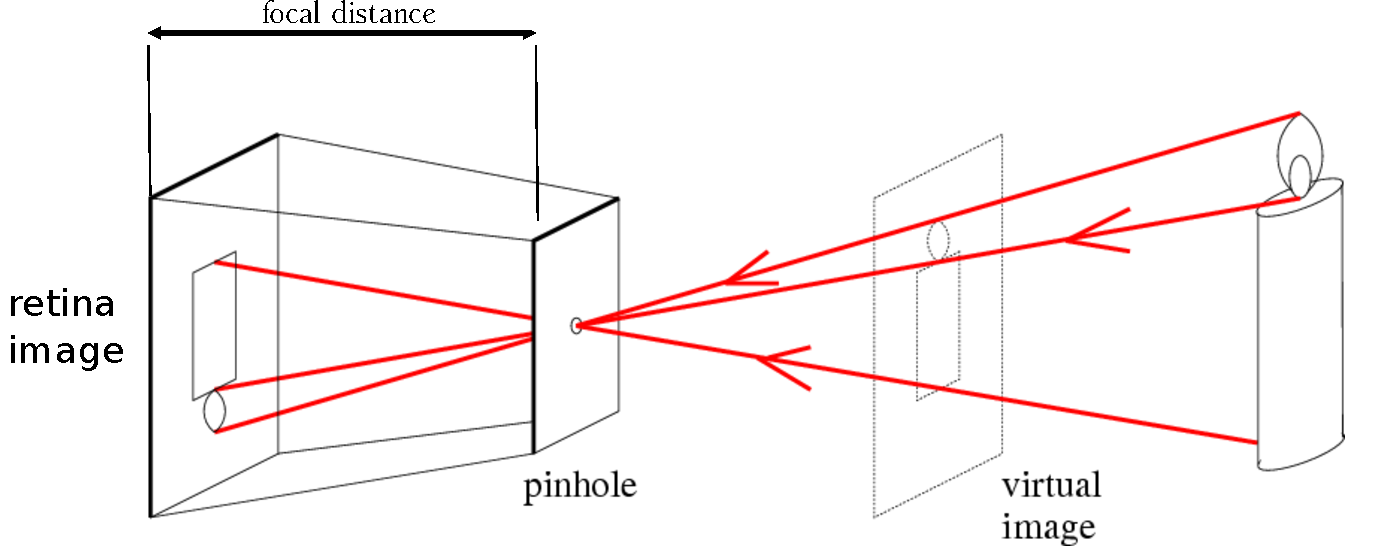
\includegraphics[width=0.6\columnwidth]{images/pinhole_camera_virtual_image.pdf}
    \end{figure}   
\end{frame}

\begin{frame}
    \frametitle{Modelo de cámara Pinhole}
    \begin{figure}[!h]
    \centering
    \subfloat[]
    {
        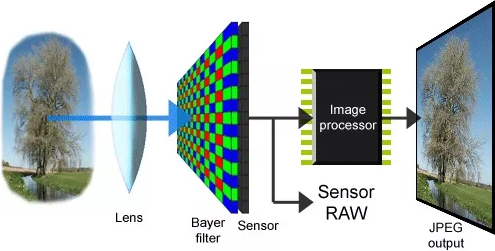
\includegraphics[width=0.55\columnwidth]{images/camera_sensor.png}
    }
    \subfloat[]
    {
        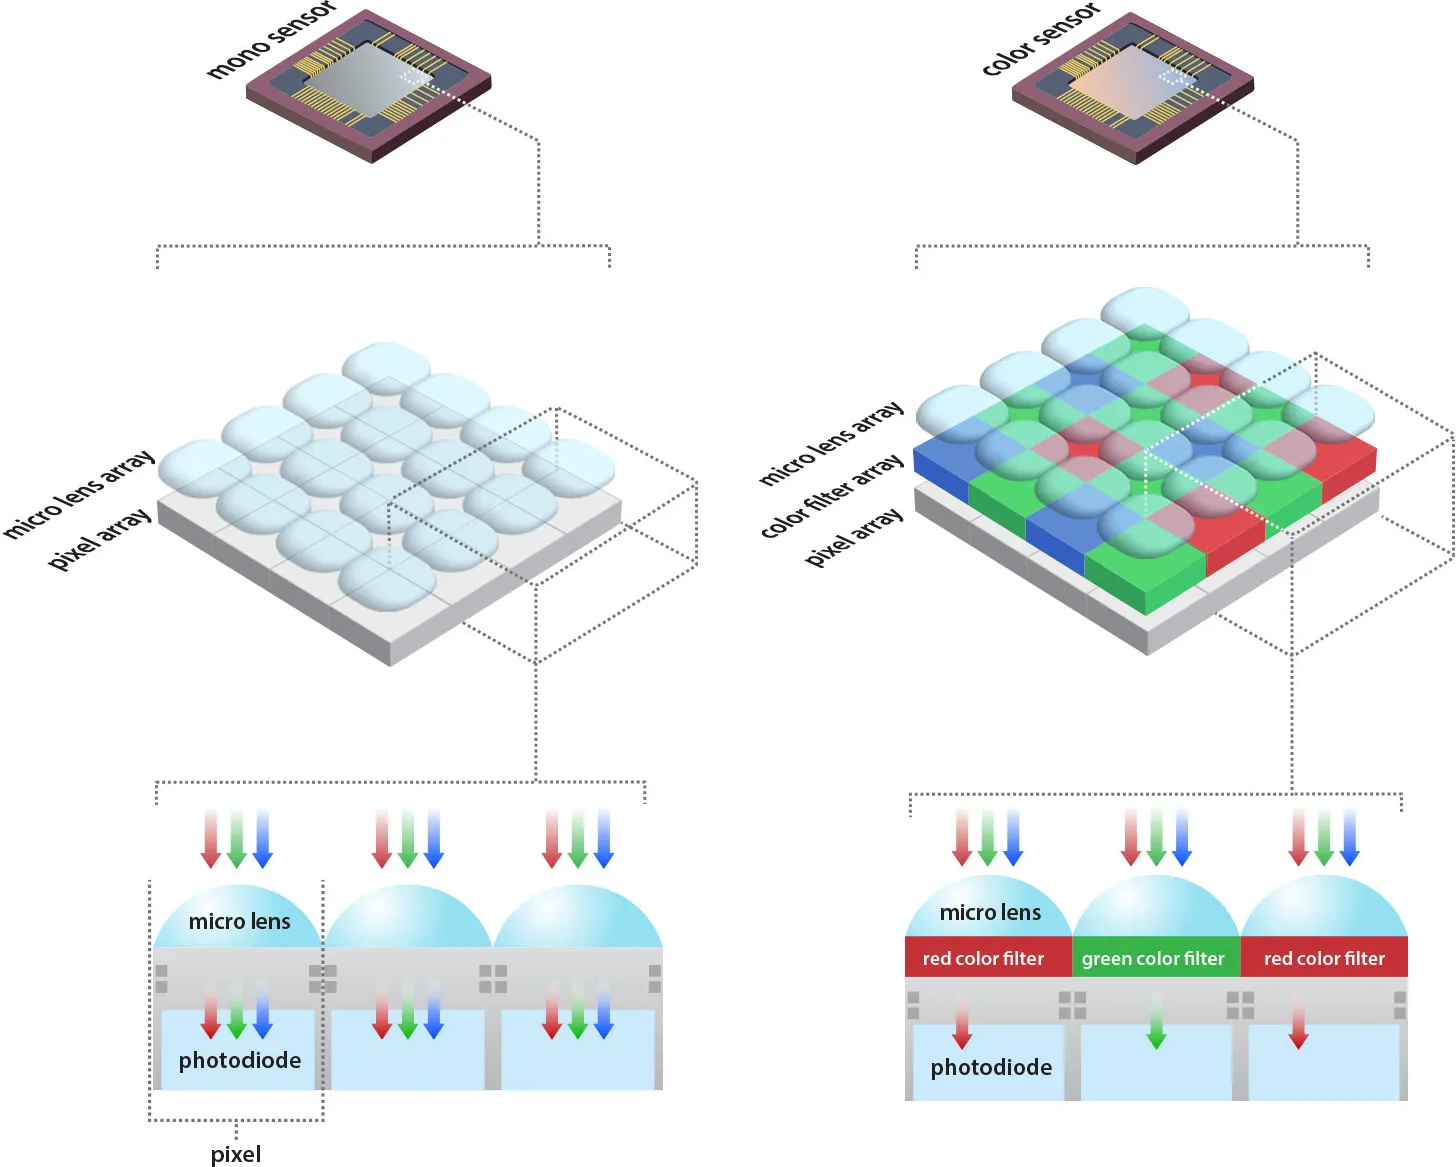
\includegraphics[width=0.4\columnwidth]{images/camera_color_mono_bayer_pattern.png}
    }
\end{figure}

\end{frame}


\begin{frame}
    \frametitle{Imagen}
    
    \begin{columns}
    	\begin{column}{0.5\textwidth}
		    \begin{figure}[!h]
			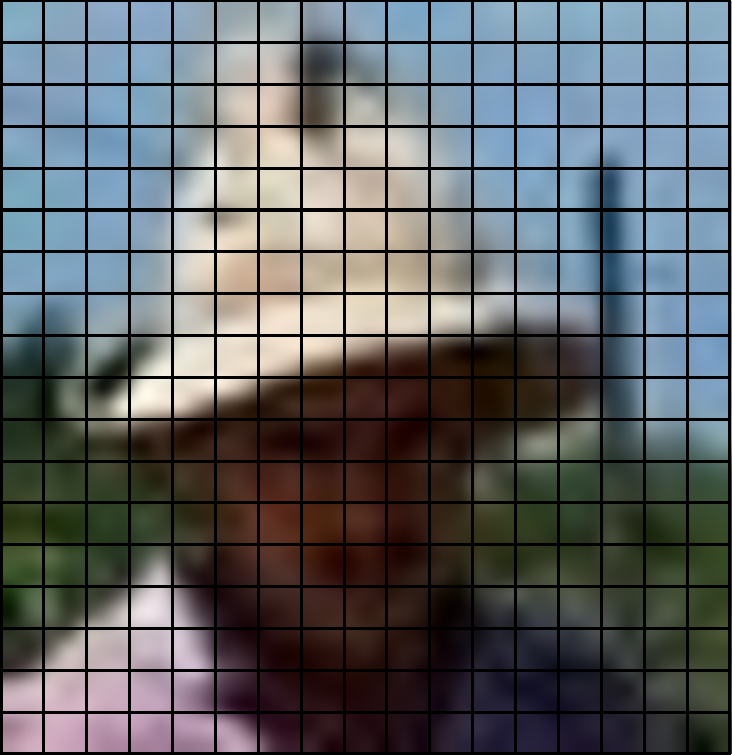
\includegraphics[width=0.6\columnwidth]{images/image_pixels.pdf}
			\end{figure}
    	\end{column}
    	\begin{column}{0.3\textwidth}
		Imagen color tiene 3 canales: R, G y B.
		\begin{equation*}
			f(x,y)=
			\begin{bmatrix}
				r(x,y) \\
				g(x,y) \\
				b(x,y)
			\end{bmatrix}
		\end{equation*}
    	\end{column}
    \end{columns}
\end{frame}

